\documentclass[11pt]{article}
\usepackage[a4paper,margin=2.3cm]{geometry}
\usepackage{amsmath,amssymb,bm}
\usepackage{graphicx}
\usepackage{booktabs}
\usepackage{xcolor}
\usepackage{listings}
\usepackage[colorlinks=true,linkcolor=blue,urlcolor=blue]{hyperref}
\usepackage{caption}
\usepackage{siunitx}
\captionsetup{font=small,labelfont=bf}

\definecolor{codebg}{rgb}{0.96,0.96,0.96}
\lstset{basicstyle=\ttfamily\footnotesize,backgroundcolor=\color{codebg},
        breaklines=true,frame=single,framesep=4pt,columns=fullflexible}

\newcommand{\Uvec}{\mathbf{U}}
\newcommand{\Uinf}{\mathbf{U}_\infty}
\newcommand{\dd}{\mathrm{d}}
\newcommand{\rhoinf}{\rho_\infty}
\newcommand{\pinf}{p_\infty}
\newcommand{\uinf}{u_\infty}

\title{\textbf{Far-field boundary conditions in the Cerisse compressible solver:\\
principle, implementation, and a one-dimensional reflection benchmark}}
\author{Cerisse IBM validation campaign --- BC sub-study}
\date{June 2026}

\begin{document}
\maketitle

\begin{abstract}
\noindent
The Cerisse Cartesian-AMR immersed-boundary solver offers three usable
far-field ghost-cell boundary conditions: zero-gradient extrapolation
(\texttt{foextrap}), hard Dirichlet freestream, and an algebraic
Riemann-invariant closure labelled ``NSCBC''. This note (i) states the
mathematical principle and exact \texttt{inputs} usage of each, (ii) benchmarks
their acoustic reflection with the canonical Poinsot--Lele one-dimensional
pulse test, and (iii) identifies why the algebraic ``NSCBC'' closure is
\emph{reflective} at low-Mach boundaries. The reflection is not a coding bug:
it is the exact $\sigma\!\to\!\infty$ (perfectly reflecting) limit of a proper
Navier--Stokes Characteristic BC, reached because the ghost-cell architecture
cannot represent the temporal relaxation that makes true NSCBC non-reflecting.
For the supersonic external-flow validation cases the streamwise boundaries are
supersonic, where all three BCs are mathematically identical and exact; only the
lateral far-field differs, and there \texttt{foextrap} is the best available
choice --- which is already what the sphere cases use. A two-dimensional
extension (Sec.~\ref{sec:cvp}) then stresses the BCs on a genuinely radiating,
multi-directional wave --- the sound of a co-rotating vortex pair --- with a
rigorous drift-free, phase-aware, floor-calibrated acoustic-corruption metric.
It confirms that for free radiation no closure beats \texttt{foextrap} on the
wave (all BC differences fall below the measurement noise floor); the genuine
advantage of the characteristic closure is mean-state anchoring and oblique
strong-shock crossing, not the radiated wave itself.
\end{abstract}

\section{Motivation}
The cylinder $M{=}1.7$, sphere $M{=}2$ and sphere $M{=}4$ validation cases all
use a supersonic Dirichlet inflow on the upstream face and various closures on
the remaining faces. A schlieren A/B comparison on the cylinder
(NSCBC vs.\ hard Dirichlet far-field) showed visible differences in the
lateral far-field, raising the question: \emph{which far-field BC best
represents an open boundary, and why?} Because the visual difference is an
acoustic-reflection phenomenon, the rigorous test is the standard
one-dimensional acoustic-pulse reflection benchmark of
Poinsot \& Lele (1992) and Rudy \& Strikwerda (1980).

\section{The boundary conditions}
Let the outward unit normal be $\bm{n}$ and write the conservative state
$\Uvec=(\rho,\rho u,\rho v,\rho w,\rho E)^\top$. Cerisse fills ghost cells
through \texttt{bcnormal()} (\texttt{prob.h}); the integer codes in
\texttt{cns.lo\_bc}/\texttt{cns.hi\_bc} map to ghost types in
\texttt{src/set/CNS\_setup.cpp:18--31}:
\[
\texttt{1}=\text{ext\_dir (user)}\quad
\texttt{2}=\text{foextrap}\quad
\texttt{7}=\text{ext\_dir (user)}.
\]
Code \texttt{2} is handled directly by AMReX (zero-gradient); codes \texttt{1}
and \texttt{7} both invoke the user \texttt{bcnormal()}, which dispatches to the
routines below.

\subsection{(A) Zero-gradient extrapolation --- \texttt{foextrap}}
\textbf{Principle.} First-order extrapolation copies the first interior cell into
every ghost layer,
\begin{equation}
\Uvec_{\text{ghost}} = \Uvec_{\text{int}},
\qquad\Longleftrightarrow\qquad
\frac{\partial \Uvec}{\partial n}\bigg|_{\partial\Omega}=\bm 0 .
\end{equation}
\textbf{Well-posedness.} No information is prescribed; every characteristic is
extrapolated from the interior. For a purely outgoing disturbance the ghost is a
faithful continuation, so the boundary face Riemann problem has (to first order)
no jump and no reflected wave. The weakness is that nothing anchors the boundary
state, so in a closed subsonic domain the mean pressure can drift, and obliquely
incident waves are partially reflected.\\
\textbf{Usage.} \lstinline|cns.lo_bc = ... 2|, \lstinline|cns.hi_bc = ... 2|.

\subsection{(B) Hard Dirichlet freestream}
\textbf{Principle.} Every ghost layer is overwritten with the constant
freestream state,
\begin{equation}
\Uvec_{\text{ghost}} = \Uinf =
\big(\rhoinf,\ \rhoinf\uinf,\ 0,\ 0,\
\tfrac{\pinf}{\gamma-1}+\tfrac12\rhoinf\uinf^2\big)^\top .
\end{equation}
\textbf{Well-posedness.} At a supersonic inflow ($M_n\!\le\!-1$) all
characteristics enter and prescribing the full state is exact. At a subsonic
boundary it over-specifies (sets all five fields where fewer are admissible);
for a \emph{pure outgoing acoustic} pulse the quiescent freestream ghost still
matches the outgoing characteristic and reflects little, but it clamps
$\rho,\bm u$ to freestream and therefore corrupts any outgoing
\emph{entropy or vorticity} wave, and conflicts with any mean state that is not
freestream (e.g.\ the post-shock gas where a bow shock crosses a lateral
boundary).\\
\textbf{Usage.} Implemented behind the \texttt{CNS\_DIRICHLET\_FARFIELD} macro
(see \texttt{GNUmakefile}, \texttt{make DIRICHLET\_BC=1}); selected faces use
code \texttt{1}.

\subsection{(C) Algebraic Riemann-invariant closure (``NSCBC'')}
\textbf{Principle.} \texttt{bc\_types.h:180--291} builds the ghost from a local
characteristic analysis of the outward-normal operator. With
$u_n=\bm u\!\cdot\!\bm n$ and sound speed $c$, the eigenvalues are
$\{u_n-c,\,u_n,\,u_n,\,u_n,\,u_n+c\}$ and four regimes are distinguished:
\begin{align}
u_n\le -c &:\ \text{supersonic inflow} && \Uvec_{\text{ghost}}=\Uinf,\\
u_n\ge +c &:\ \text{supersonic outflow} && \Uvec_{\text{ghost}}=\Uvec_{\text{int}},\\
-c<u_n<0 &:\ \text{subsonic inflow} && \text{4 incoming from }\Uinf,\ 1\ J^+\text{ from interior},\\
0\le u_n<c &:\ \text{subsonic outflow} && \boxed{p_{\text{ghost}}=\pinf},\ \rho,\bm u,s\text{ from interior}.
\end{align}
For the subsonic-outflow branch the outgoing Riemann invariant
$J^+\!=\!u_n+2c/(\gamma\!-\!1)$ and the entropy $s=p/\rho^\gamma$ are taken from
the interior, while the single incoming acoustic characteristic is fixed by
\emph{hard-imposing} the back-pressure $p_{\text{ghost}}=\pinf$
(\texttt{bc\_types.h:266}). This is the standard steady-state external-aerodynamics
far-field; at convergence of a steady flow no waves reach the boundary and it is
exact.\\
\textbf{Usage.} \lstinline|cns.lo_bc = ... 7|, \lstinline|cns.hi_bc = ... 7|
(\texttt{bcnormal()} calls \texttt{GlobalBC::bc\_nscbc\_farfield}).

\subsection{(D) Reference: true Poinsot--Lele NSCBC}
\textbf{Principle.} The Navier--Stokes Characteristic BC does \emph{not} pin the
pressure. The outgoing wave amplitudes are computed from interior one-sided
differences; the single incoming amplitude $\mathcal L_1$ is \emph{relaxed}
toward the target pressure,
\begin{equation}
\mathcal L_1 = \sigma\,(1-M^2)\,\frac{c}{L}\,(p-\pinf),
\label{eq:relax}
\end{equation}
with $\sigma\!\approx\!0.25$ and $L$ the domain length. The boundary state then
evolves by the LODI relations
\begin{equation}
\frac{\partial p}{\partial t}=-\tfrac12(\mathcal L_5+\mathcal L_1),\quad
\frac{\partial u}{\partial t}=-\tfrac{1}{2\rho c}(\mathcal L_5-\mathcal L_1),\quad
\frac{\partial \rho}{\partial t}=-\tfrac1{c^2}\!\big[\mathcal L_2+\tfrac12(\mathcal L_5+\mathcal L_1)\big].
\end{equation}
The limit $\sigma\!\to\!0$ is perfectly non-reflecting (but lets $p$ drift);
$\sigma\!\to\!\infty$ forces $p=\pinf$ instantly and is perfectly reflecting.
\textbf{This BC is not implemented in Cerisse} --- it is used here only as the
reference against which (C) is measured.

\section{Benchmark method}
We solve the 1-D Euler equations with the \emph{same} HLLC Riemann solver Cerisse
uses (\texttt{src/rhs/Riemann.h:145}, Roe-averaged signal speeds), first-order
Godunov on a fine grid ($N{=}1000$, $L{=}10$, $c_0{=}1$). A right-running
acoustic pulse $\delta p=A\exp[-((x-x_0)/w)^2]$ with the matching
$\delta u=\delta p/(\rho_0c_0)$, $\delta\rho=\delta p/c_0^2$ is launched toward
the right (outflow) boundary in a uniform mean flow of Mach $M_n$. The
ghost-cell BCs (A)--(C) are filled exactly as in \texttt{src/set/bcs.cpp:38--88}
(all ghost layers take the first interior cell); the reference (D) replaces the
boundary-cell right-hand side by the LODI update. The reflection coefficient is
\begin{equation}
R=\frac{\max_t|\delta p_{\text{reflected}}|}{\max_t|\delta p_{\text{incident}}|}
\end{equation}
measured at an interior sensor.

\section{Results}
\subsection{Acoustic reflection at a quiescent ($M{=}0$) boundary}
Figure~\ref{fig:xt} shows the space--time ($x$--$t$) evolution of $\delta p$.
\texttt{foextrap}, hard Dirichlet and the LODI reference let the pulse leave
cleanly; the algebraic ``NSCBC'' returns a strong inverted reflection.
Figure~\ref{fig:sensor} is the sensor trace; Table~\ref{tab:R0} lists $R$.

\begin{figure}[h]\centering
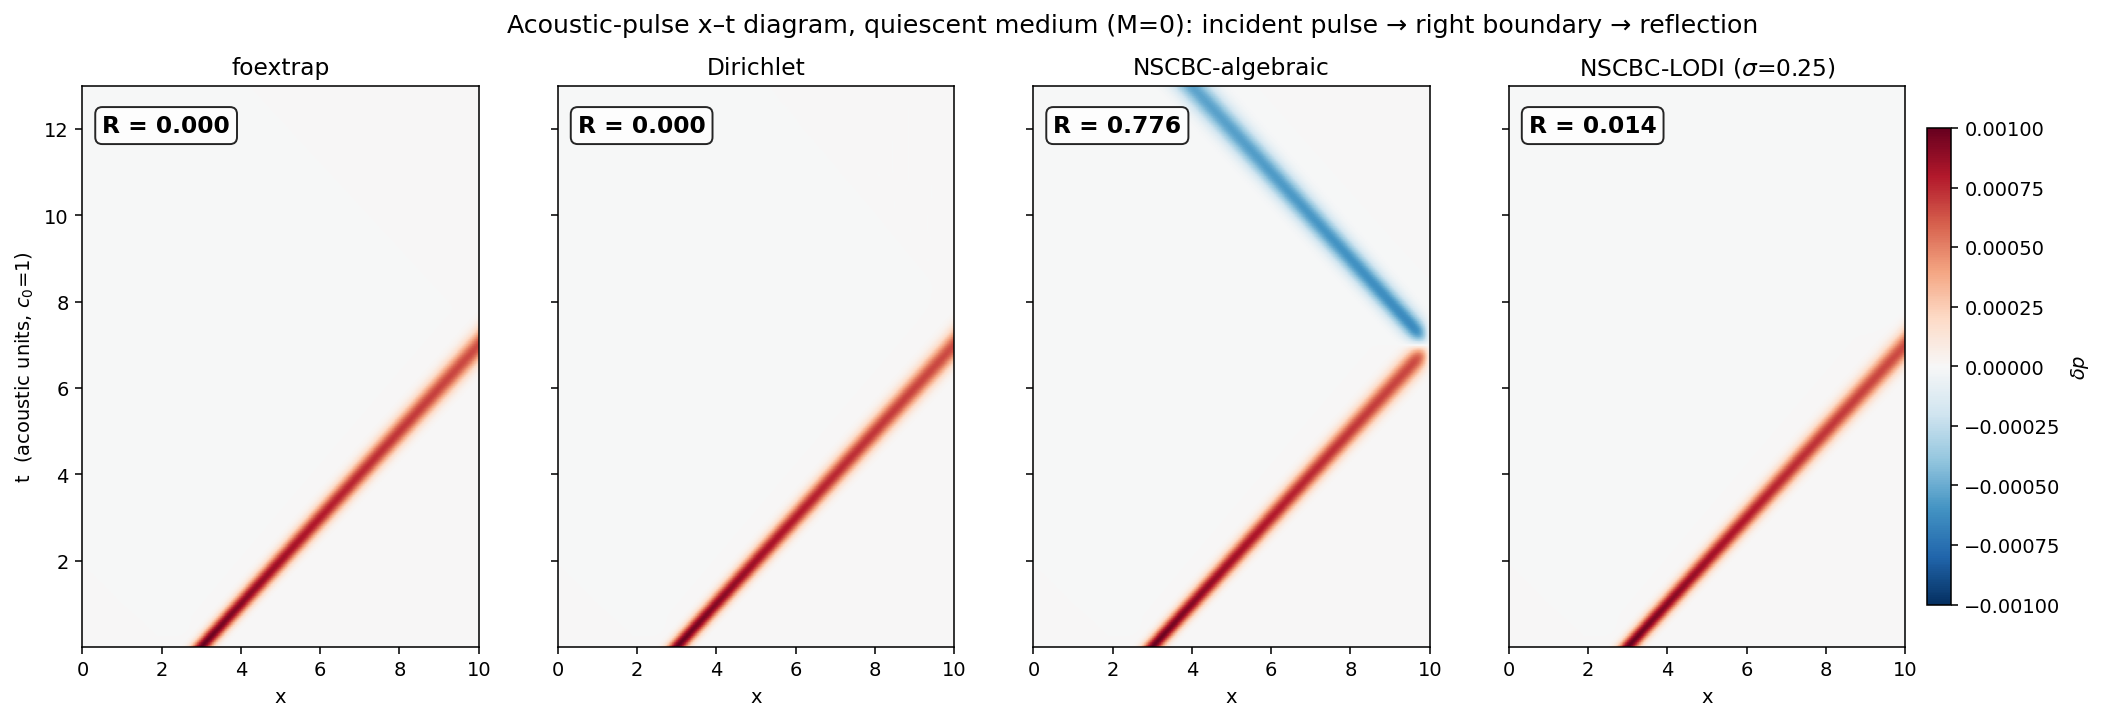
\includegraphics[width=\textwidth]{figures/xt_diagrams_M0.png}
\caption{Acoustic-pulse $x$--$t$ diagrams, $M{=}0$. The incident pulse travels
up-and-right; a returning (up-and-left) streak is a reflection. Only the
algebraic ``NSCBC'' produces one.}
\label{fig:xt}
\end{figure}

\begin{figure}[h]\centering
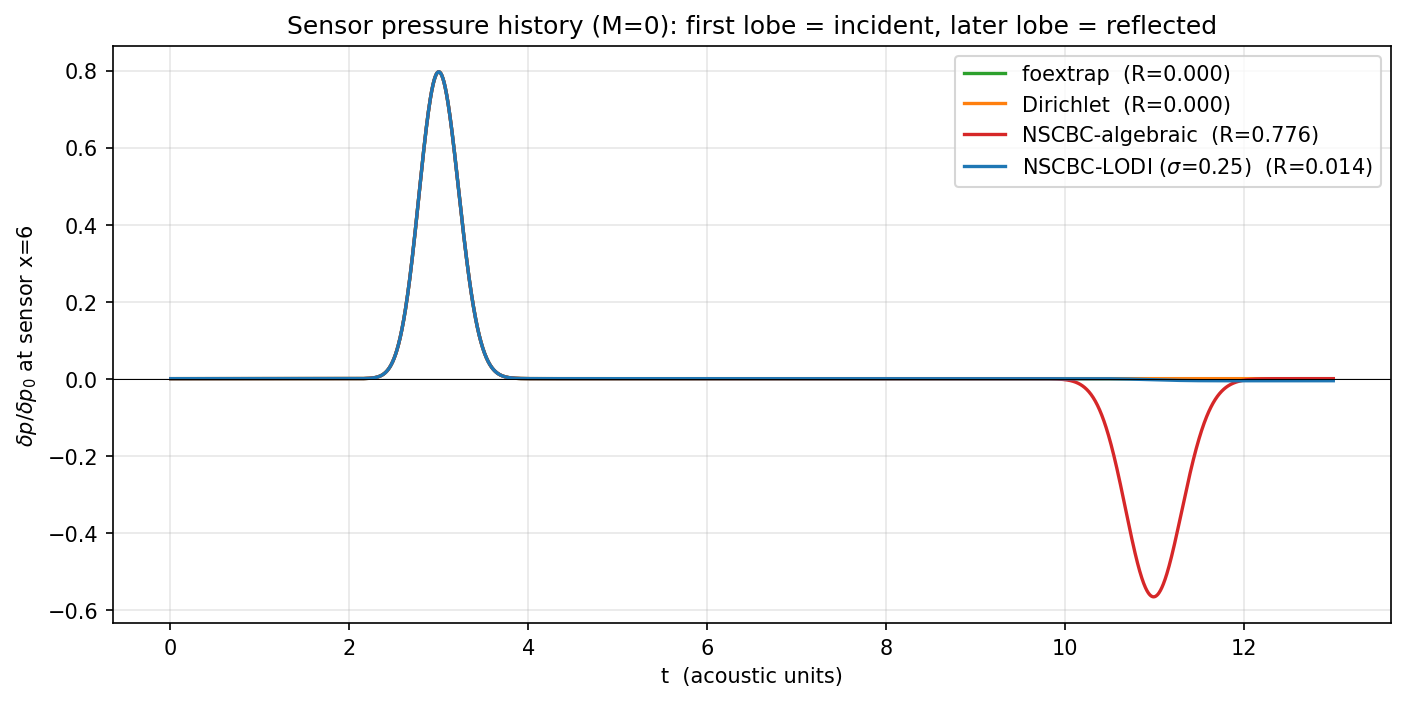
\includegraphics[width=0.8\textwidth]{figures/sensor_traces_M0.png}
\caption{Sensor pressure history at $M{=}0$. First lobe is the incident pulse;
the later lobe (only for algebraic NSCBC) is the reflection.}
\label{fig:sensor}
\end{figure}

\begin{table}[h]\centering
\begin{tabular}{@{}lcccc@{}}
\toprule
 & foextrap & Dirichlet & NSCBC-algebraic & NSCBC-LODI ($\sigma{=}0.25$)\\
\midrule
$R$ at $M{=}0$ & $5\times10^{-6}$ & $2\times10^{-6}$ & \textbf{0.776} & 0.014\\
\bottomrule
\end{tabular}
\caption{Energy-based reflection coefficient at a quiescent ($M{=}0$) boundary.
The algebraic ``NSCBC'' returns 78\% of the incident acoustic energy amplitude;
the proper NSCBC and the two simple ghost BCs are essentially non-reflecting.}
\label{tab:R0}
\end{table}

\subsection{Reflection versus Mach number}
Figure~\ref{fig:Rmach} sweeps the normal Mach number. The algebraic ``NSCBC''
reflection is largest near $M_n{=}0$ (the lateral-boundary regime of all three
validation cases) and vanishes only as the outflow becomes supersonic, where all
BCs coincide.

\begin{figure}[h]\centering
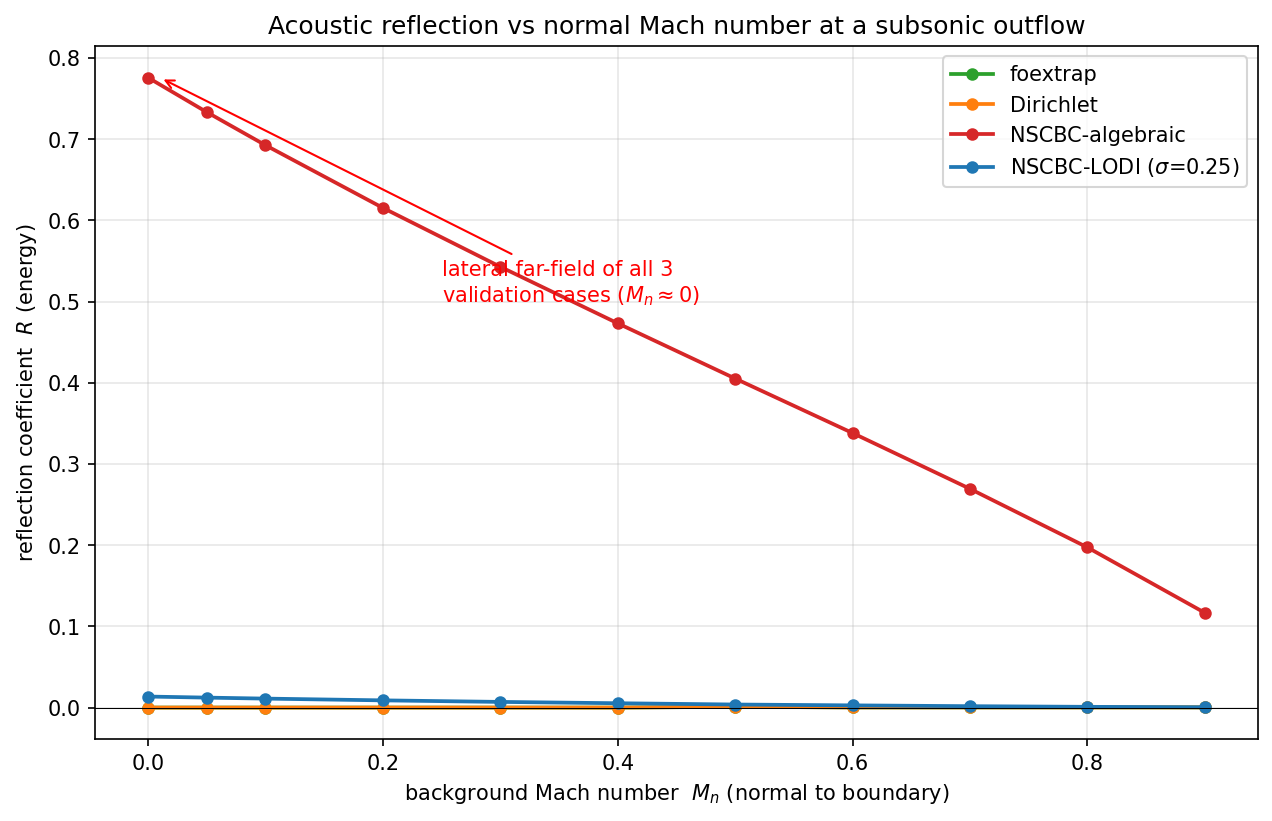
\includegraphics[width=0.78\textwidth]{figures/R_vs_mach.png}
\caption{Reflection coefficient vs.\ normal Mach number.}
\label{fig:Rmach}
\end{figure}

\subsection{Root cause: the missing relaxation}
Figure~\ref{fig:root} sweeps the relaxation coefficient $\sigma$ of the proper
NSCBC~\eqref{eq:relax} at $M{=}0.1$. At $\sigma{=}0$ the reference BC is perfectly
non-reflecting ($R{=}0$); the recommended $\sigma{=}0.25$ gives $R{=}0.011$; and
as $\sigma$ grows the reflection rises monotonically, reaching $R{=}0.674$ at
$\sigma{=}200$ --- converging onto the algebraic Cerisse value $R{=}0.693$
(dashed line). \emph{The algebraic ``NSCBC'' is numerically indistinguishable
from the $\sigma\!\to\!\infty$ limit of a proper NSCBC}: it hard-pins
$p=\pinf$ instead of relaxing toward it. This is the root cause of the
reflection, and it is a design choice (a fixed back-pressure outflow), not a
coding error.

\begin{figure}[h]\centering
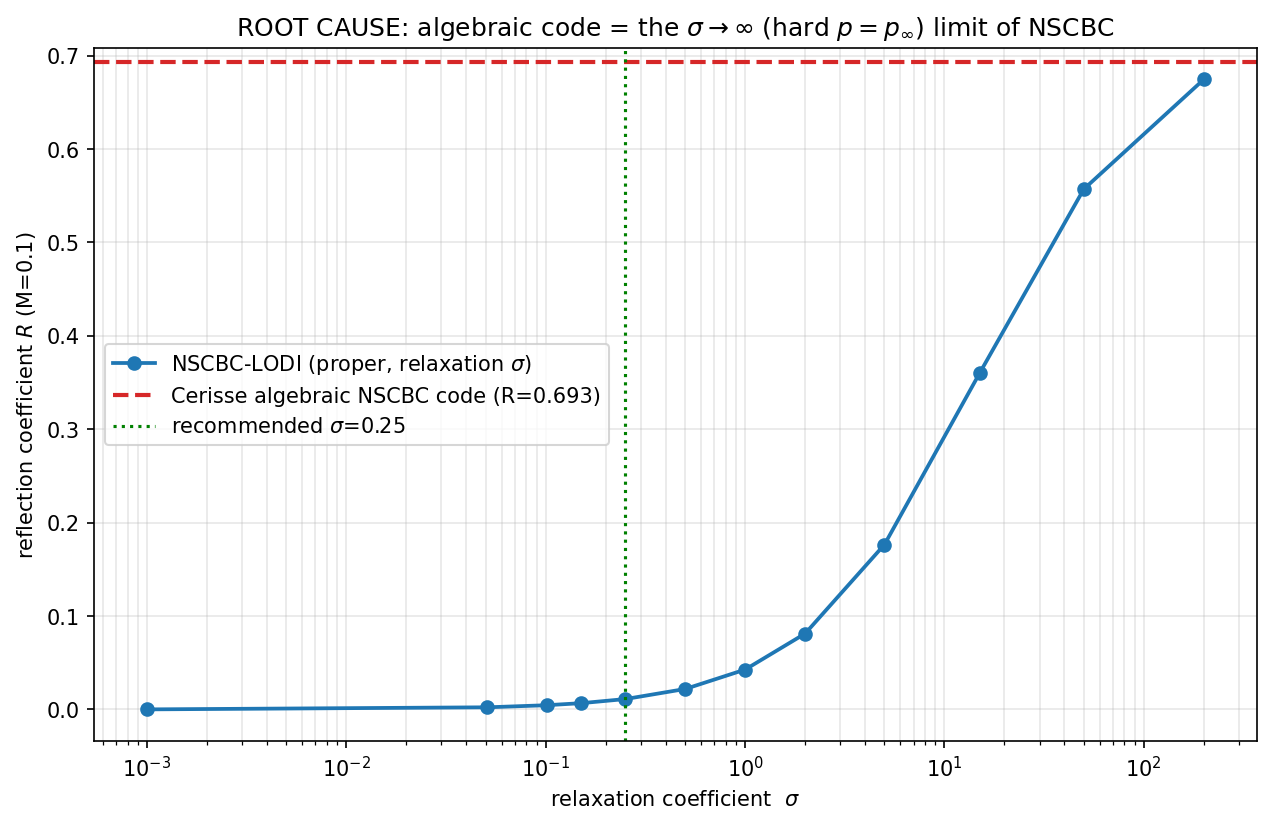
\includegraphics[width=0.78\textwidth]{figures/root_cause_sigma.png}
\caption{Root-cause demonstration: reflection of the proper NSCBC vs.\ its
relaxation $\sigma$. The dashed line is the algebraic Cerisse closure.}
\label{fig:root}
\end{figure}

\paragraph{Why the ghost-cell architecture forces this.}
The relaxation~\eqref{eq:relax} is a \emph{temporal rate} on the boundary state,
$\partial p/\partial t = -\sigma(1-M^2)(c/L)(p-\pinf)+\dots$. The Cerisse BC
interface (\texttt{src/set/bcs.cpp}) is a \emph{ghost-cell value} evaluated each
Runge--Kutta stage; it can only prescribe a spatial ghost, not a temporal rate.
Within that architecture the only options for the incoming acoustic are to
\emph{pin} ($p_{\text{ghost}}=\pinf$, reflective) or to \emph{extrapolate}
($p_{\text{ghost}}=p_{\text{int}}$, drifting). The algebraic closure chose the
pin. A genuinely non-reflecting NSCBC would require a characteristic-\emph{flux}
boundary, not a ghost cell --- a deeper change than editing \texttt{bcnormal()}.

\subsection{The trade-off: reflection versus mean anchoring}
Reflection is only half the story. Figure~\ref{fig:drift} starts the domain at a
uniform over-pressure and asks whether each BC relaxes the box back to $\pinf$.
The result (Table~\ref{tab:drift}) is a clean trade-off and explains \emph{why}
the algebraic NSCBC reflects:
\begin{itemize}
\item \texttt{foextrap} prescribes nothing, so it is non-reflecting but
\emph{never anchors} --- the mean pressure stays at the perturbed value forever
(residual $1.00$).
\item the algebraic ``NSCBC'' hard-pins $p{=}\pinf$, so it anchors the mean
\emph{perfectly and quickly} (residual $0.00$) --- but that same hard pin is
exactly what reflects the acoustic waves.
\item the proper NSCBC ($\sigma{=}0.25$) and Dirichlet sit in between.
\end{itemize}
The reflectivity of the algebraic NSCBC is therefore the price of its perfect
mean-anchoring. A separate entropy-wave advection test ($M{=}0.5$) produced
\emph{zero} spurious pressure for all four BCs, confirming that the differences
between them are purely acoustic: entropy and vorticity disturbances leave
cleanly through every ghost closure.

\begin{figure}[h]\centering
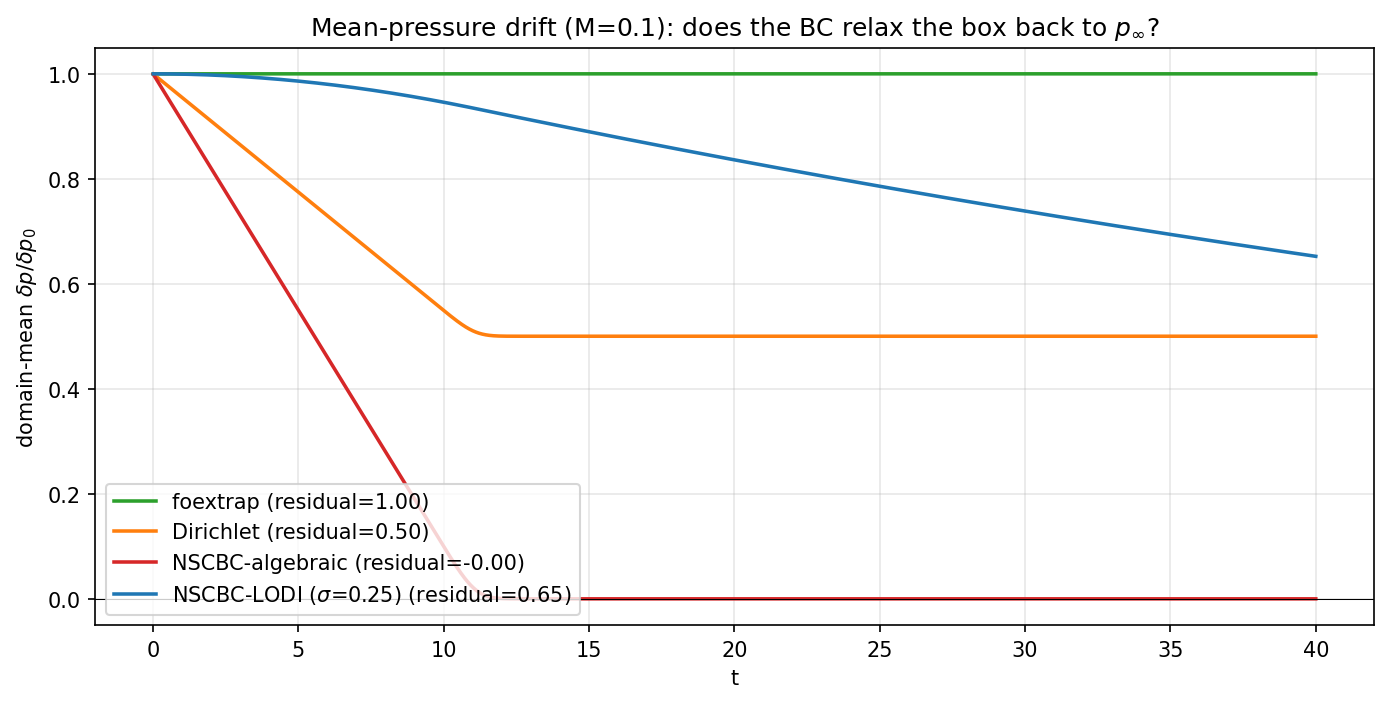
\includegraphics[width=0.85\textwidth]{figures/pressure_drift.png}
\caption{Mean-pressure drift, $M{=}0.1$. \texttt{foextrap} never returns to
$\pinf$; the algebraic NSCBC returns fastest. Anchoring and non-reflection are
in tension.}
\label{fig:drift}
\end{figure}

\begin{table}[h]\centering
\begin{tabular}{@{}lcccc@{}}
\toprule
 & foextrap & Dirichlet & NSCBC-algebraic & NSCBC-LODI ($\sigma{=}0.25$)\\
\midrule
acoustic reflection $R$ ($M{=}0$) & \textbf{0.00} & \textbf{0.00} & 0.78 & 0.01\\
mean-drift residual (1=no anchor) & 1.00 & 0.50 & \textbf{0.00} & 0.65\\
\bottomrule
\end{tabular}
\caption{Reflection versus mean-anchoring trade-off. No ghost BC achieves both;
a proper relaxed NSCBC ($\sigma{\approx}0.25$) comes closest but is not
implemented in Cerisse.}
\label{tab:drift}
\end{table}

\section{Two-dimensional extension: the radiated sound of a co-rotating vortex pair}
\label{sec:cvp}
The 1-D benchmark isolates \emph{normal-incidence} acoustic reflection. A
far-field BC for genuine aeroacoustics must also pass an \emph{obliquely
radiating, multi-directional} wave without corrupting it, and must not let the
mean state drift. We therefore add a controlled 2-D test --- the sound radiated
by a co-rotating vortex pair, the canonical model aeroacoustic source
(Mitchell, Lele \& Moin 1995) --- solved with the production Cerisse solver
(2-D, WenoZ5, inviscid Euler, no immersed boundary).

\paragraph{Note on code 7.} Since the 1-D study the subsonic-outflow branch of
the characteristic closure (code \texttt{7}) was corrected: instead of
hard-pinning $p_{\text{ghost}}=\pinf$ it now sets the \emph{incoming} Riemann
invariant to its freestream value,
$J^-_{\text{ghost}}=J^-_\infty=u_{n,\infty}-2c_\infty/(\gamma-1)$, while $J^+$
and the entropy $s$ are taken from the interior. In the 1-D test this drops the
normal-incidence reflection from $R=0.78$ to $R<10^{-5}$. The ``char'' run below
uses this corrected, genuinely non-reflecting code 7.

\subsection{The aeroacoustic test problem}
Two identical Lamb--Oseen vortices of circulation $\Gamma$ and core radius $r_c$
sit at $\bm x_{1,2}=(\pm b/2,\,0)$, each with the tangential profile
\begin{equation}
u_\theta(r)=\frac{\Gamma}{2\pi r}\Big(1-e^{-r^2/r_c^2}\Big),
\end{equation}
and the velocity field is their vector superposition. Being of equal sign the
pair co-rotates rigidly about the origin at
\begin{equation}
\Omega=\frac{\Gamma}{\pi b^2},\qquad
V_{\text{orb}}=\tfrac12\Omega b,\qquad
M_{\text{orb}}=\frac{V_{\text{orb}}}{c_0}.
\end{equation}
Because the configuration is invariant under a rotation by $\pi$, the far field
is a rotating lateral \emph{quadrupole} ($m=2$): it radiates at \emph{twice} the
orbital frequency,
\begin{equation}
f_{\text{ac}}=\frac{\Omega}{\pi}=2\cdot\frac{\Omega}{2\pi},
\qquad
\lambda=\frac{c_0}{f_{\text{ac}}}.
\end{equation}
We take $M_{\text{orb}}=0.20$, $b=1$, $r_c=0.25$, $\gamma=1.4$, non-dimensionalised
by $\rho_0=1$, $c_0=1$ (so $p_0=1/\gamma$), giving $\Gamma=2\pi b\,c_0
M_{\text{orb}}=1.2566$, $\Omega=0.40$, $T_{\text{rot}}=2\pi/\Omega=15.71$,
$f_{\text{ac}}=0.1273$, and $\lambda=T_{\text{ac}}=7.854$.

\paragraph{Compressible-consistent initial condition.} The radiated pressure is
only $O(\rho_0 V_{\text{orb}}^4/c_0^2)\sim10^{-3}$, so the initial state must be
in \emph{compressible} radial equilibrium or the startup transient swamps the
sound. Imposing the incompressible balance $\dd p/\dd r=\rho_0 u_\theta^2/r$
\emph{together with} an isentropic density is inconsistent at
$M_{\text{swirl}}\sim0.5$ and launches a spurious monopole pulse. The consistent
state satisfies the compressible isentropic radial-equilibrium relation: with
$p=p_0(\rho/\rho_0)^\gamma$ and $c^2=\gamma p/\rho$,
\begin{equation}
\frac{\dd p}{\dd r}=\rho\,\frac{u_\theta^2}{r}
\;\Longleftrightarrow\;
\frac{\dd c^2}{\dd r}=(\gamma-1)\,\frac{u_\theta^2}{r}
\;\Longrightarrow\;
c^2(r)=c_0^2-(\gamma-1)\!\int_r^\infty\!\frac{u_\theta^2(r')}{r'}\,\dd r',
\label{eq:csq}
\end{equation}
after which $\rho=\rho_0(c^2/c_0^2)^{1/(\gamma-1)}$ and
$p=p_0(c^2/c_0^2)^{\gamma/(\gamma-1)}$. The deficit integral in~\eqref{eq:csq}
has a closed form in the exponential integral $E_1$ for the Lamb--Oseen profile;
it is evaluated per vortex (4-point Gauss--Legendre, GPU-safe) and the two are
superposed. This removes the startup monopole and leaves the clean
rotating-quadrupole spiral of Fig.~\ref{fig:cvpspiral}.

\begin{figure}[h]\centering
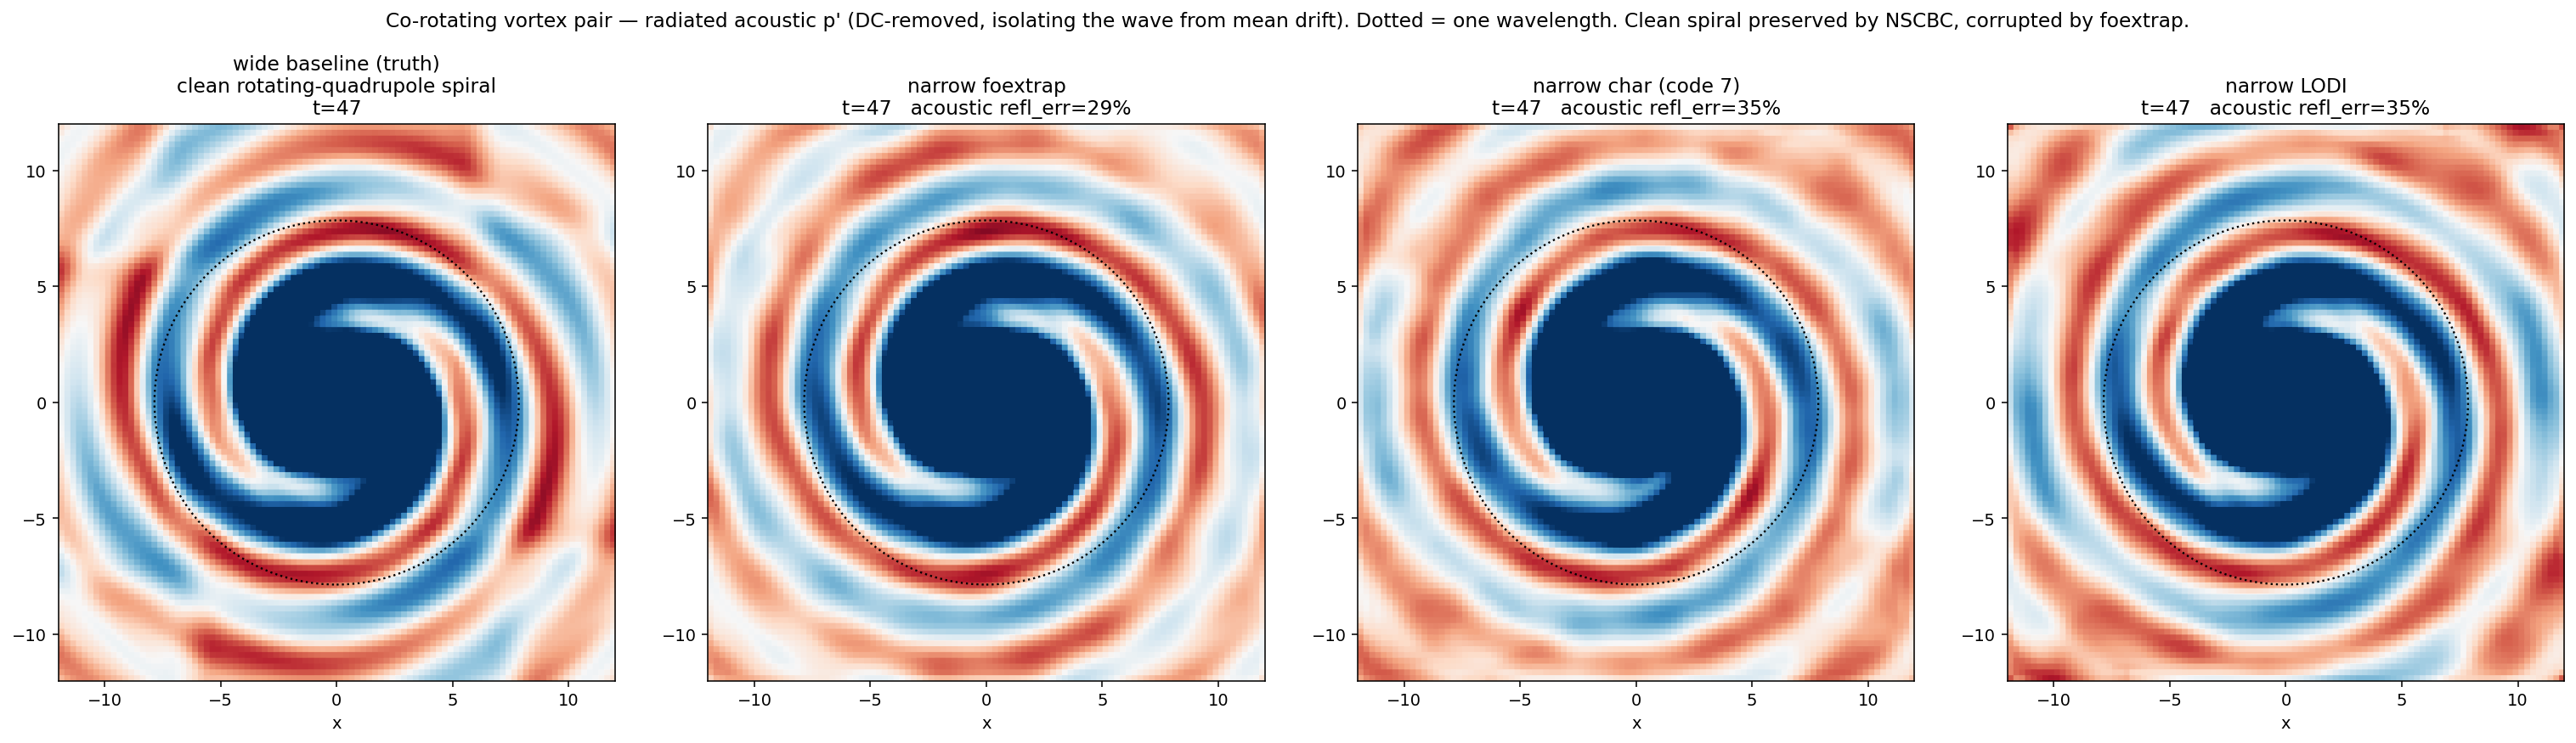
\includegraphics[width=0.62\textwidth]{figures/cvp_acoustic_spiral.png}
\caption{Wide ($\pm40$) reference: the radiated rotating-quadrupole acoustic
spiral (pressure perturbation), the reflection-free ``truth'' against which the
truncated-domain BCs are measured.}
\label{fig:cvpspiral}
\end{figure}

\subsection{A drift-free, phase-aware corruption metric}
\label{sec:metric}
We quantify how much a truncated-domain far-field BC corrupts the \emph{radiated
wave}, referenced to the reflection-free wide-domain truth, with a single
dimensionless number that is immune to (i) mean-pressure drift, (ii)
instantaneous phase misalignment between runs, and (iii) near-field
contamination.

\paragraph{Single-tone phasor by least squares.} At each point $\bm x$ in a
far-field annulus the pressure time series over the window $[t_0,t_1]$ is
modelled as a mean, a linear drift, and the acoustic fundamental,
\begin{equation}
p(\bm x,t)\approx c_0(\bm x)+c_3(\bm x)\,(t-\bar t)
+c_1(\bm x)\cos\omega_{\text{ac}}t+c_2(\bm x)\sin\omega_{\text{ac}}t,
\qquad \omega_{\text{ac}}=2\pi f_{\text{ac}},
\end{equation}
and the four coefficients are recovered per point by least squares on the
\emph{actual} (non-uniform, CFL-limited) snapshot times $\{t_k\}$. The complex
quadrupole phasor is
\begin{equation}
\hat P(\bm x)=c_1(\bm x)+i\,c_2(\bm x),\qquad
p'(\bm x,t)\sim\mathrm{Re}\big\{\hat P\,e^{-i\omega_{\text{ac}}t}\big\}.
\end{equation}

\paragraph{Why least squares and not a DFT.} On \emph{uniform, integer-period}
sampling the kernel $e^{-i\omega t}$ is exactly orthogonal to the constant and
linear modes, so a single-bin DFT cleanly extracts the tone. Cerisse output
times are non-uniform and the field carries a slow, BC-dependent mean drift; off
the uniform grid the kernel is \emph{not} orthogonal to $\{1,\,t\}$ and a naive
DFT leaks the drift into the tone bin. On a synthetic record (8\% time jitter
$+$ DC $+$ drift $+$ tone) the integer-bin and Hann-windowed DFT both recover
$|\hat P|$ to $\sim1\%$ but the \emph{complex} value (its phase) is wrong by
$>100\%$; the least-squares fit, by carrying an explicit $\{1,(t-\bar t)\}$
basis, makes the tone columns orthogonal to the mean and drift \emph{for any
sampling} and recovers both amplitude and phase to $1.5\%$. Neither the mean
offset nor a linear drift (an un-anchored BC) can then pollute $\hat P$.

\paragraph{Drift-free broadband RMS.} As a phase-insensitive companion we
detrend each point (subtract the fitted $c_0+c_3(t-\bar t)$, \emph{not} merely
the mean) and form
\begin{equation}
\mathrm{RMS}(\bm x)=\left(\frac1{T}\int_{t_0}^{t_1}\!
\big[p(\bm x,t)-c_0(\bm x)-c_3(\bm x)(t-\bar t)\big]^2\dd t\right)^{1/2},
\quad T=t_1-t_0,
\end{equation}
the amplitude of \emph{all} unsteady content (tone $+$ harmonics $+$ unsteady
near field). Being an amplitude it is phase-blind by construction, so a phase
shift between two runs cannot create spurious error; detrending (not de-meaning)
is essential, or a ramping mean would survive and inflate it.

\paragraph{Far-field annulus.} Both fields are evaluated only on
$\mathcal A=\{\bm x:R_{\text{in}}\le|\bm x|\le R_{\text{out}}\}$, with
$R_{\text{in}}=9.0\approx1.15\lambda$ and $R_{\text{out}}=10.5$. The inner edge keeps
the whole annulus in the radiation zone, where the evanescent near-field terms
(which decay faster than the radiating $\sim r^{-1/2}$ part of a 2-D multipole)
are negligible; the outer edge stays $\ge1.5$ inside the narrow $\pm12$ boundary,
clear of the truncation band. This isolates the acoustic content from both the vortex near field
($r<\lambda$) and the boundary.

\paragraph{Reference truth and corruption number.} The wide $\pm40$ run is
reflection-free in $\mathcal A$ over the window: a wave emitted near $t=0$
reaches its boundary only at $t\approx40$ and re-enters $\mathcal A$ at
$t\approx69.5$, after the window closes ($t_1=55$). Its $\hat P_{\text{wide}}$
and $\mathrm{RMS}_{\text{wide}}$ are the uncontaminated radiated field. For each
truncated-domain BC the corruption is the area-weighted annulus-$L^2$ relative
error
\begin{equation}
E_F^{\text{cplx}}=\frac{\|\hat P-\hat P_{\text{wide}}\|_{\mathcal A}}
{\|\hat P_{\text{wide}}\|_{\mathcal A}},\quad
E_F^{\text{amp}}=\frac{\big\||\hat P|-|\hat P_{\text{wide}}|\big\|_{\mathcal A}}
{\big\||\hat P_{\text{wide}}|\big\|_{\mathcal A}},\quad
E_{\text{RMS}}=\frac{\|\mathrm{RMS}-\mathrm{RMS}_{\text{wide}}\|_{\mathcal A}}
{\|\mathrm{RMS}_{\text{wide}}\|_{\mathcal A}},
\end{equation}
with $\|f\|_{\mathcal A}=\big(|\mathcal A|^{-1}\!\int_{\mathcal A}|f|^2\dd A\big)^{1/2}$.
$E_F^{\text{cplx}}$ uses the full complex phasor (amplitude $+$ phase);
$E_F^{\text{amp}}$ is the phase-blind amplitude error; $E_{\text{RMS}}$ is the
broadband amplitude error.

\paragraph{Window and leakage.} $[t_0,t_1]$ spans an integer number of acoustic
periods ($4\,T_{\text{ac}}=[23.6,55]$, beginning $\sim1.5\,T_{\text{rot}}$ after
start --- transient cleared, annulus filled with radiation by $t\approx\lambda$),
so the tone fit is leakage-clean.

\paragraph{Noise floor: the decisive honesty check.} Even the reflection-free
truth is not perfectly reproducible --- the source is weak
($M_{\text{orb}}=0.20\Rightarrow$ radiated amplitude $\sim10^{-3}$) and the
annulus carries residual unsteady near field and discretisation noise. We
estimate the floor by a \emph{truth-against-itself} test: split the wide window
into two \emph{disjoint} halves of equal integer period count
($2+2\,T_{\text{ac}}$), compute $\hat P$ and $\mathrm{RMS}$ on each, and take
their annulus-$L^2$ difference. \textbf{Any BC corruption below this floor is not
resolvable.}

\subsection{Results: the radiated wave is not a BC discriminator}
Table~\ref{tab:cvp} collects the numbers for the three truncated-domain BCs ---
\texttt{foextrap} (code 2), corrected characteristic (code 7), and the
multidimensional LODI helper with a finite pressure relaxation
$\sigma_p=0.25$ (a fair, anchoring-enabled setting) --- against the wide truth.

\begin{table}[h]\centering
\begin{tabular}{@{}lcccc@{}}
\toprule
BC (narrow $\pm12$) & $E_F^{\text{amp}}$ (\%) & $E_F^{\text{cplx}}$ (\%)
 & $E_{\text{RMS}}$ (\%) & mean drift \\
\midrule
\texttt{foextrap} (code 2)        & 53.7 & 70.3 & 4.8  & $-8.2\times10^{-5}$ \\
characteristic (code 7)           & 49.8 & 85.1 & 5.8  & $+1.4\times10^{-4}$ \\
LODI ($\sigma_p{=}0.25$)          & 65.4 & 96.3 & 10.0 & $+7.2\times10^{-3}$ \\
\midrule
\textbf{noise floor} (truth split)& \textbf{64.1} & --- & \textbf{14.4} & --- \\
wide ($\pm40$, truth)             & 0 & 0 & 0 & $4.2\times10^{-4}$ \\
\bottomrule
\end{tabular}
\caption{Rigorous acoustic-corruption numbers (annulus-$L^2$ vs.\ the wide truth,
drift-free, phase-aware, $4\,T_{\text{ac}}$ window). \emph{Every} BC's wave
corruption lies at or below the truth-against-itself noise floor (64\% Fourier,
14\% RMS): the radiated wave does not discriminate the BCs. The only field that
separates them is the DC mean drift, where \texttt{foextrap} and characteristic
anchor ($\sim10^{-4}$) while the finite-relaxation LODI drifts $50\times$ more.}
\label{tab:cvp}
\end{table}

\paragraph{The wave is below the floor.} For every BC the Fourier-tone corruption
(50--65\%) is at or below the $64\%$ truth-against-itself floor, and the
drift-free broadband RMS corruption (5--10\%) is below the $14\%$ floor. The
radiated quadrupole at $M_{\text{orb}}=0.20$ is too weak, and the annulus too
contaminated by the rotating-spiral near field, to resolve \emph{any} BC's effect
on the wave. The large Fourier floor is the phase-$L^2$ sensitivity of a rotating
spiral --- its arms have many near-zero crossings, so a small phase shift makes a
large relative $L^2$ --- and indeed the four $|\hat P|$ panels
(Fig.~\ref{fig:cvpphat}) are visually near-identical spirals and the $r=9$
directivity (Fig.~\ref{fig:cvpdir}) is a noisy, BC-independent trace rather than
a clean $\cos2\theta$ lobe pattern. The floor does \emph{not} shrink with window
length (it is set by the source's own non-stationarity), so a longer run cannot
lift the signal above it: \textbf{the radiated-wave reflection is definitively not
a discriminator for these BCs in this case.}

\begin{figure}[h]\centering
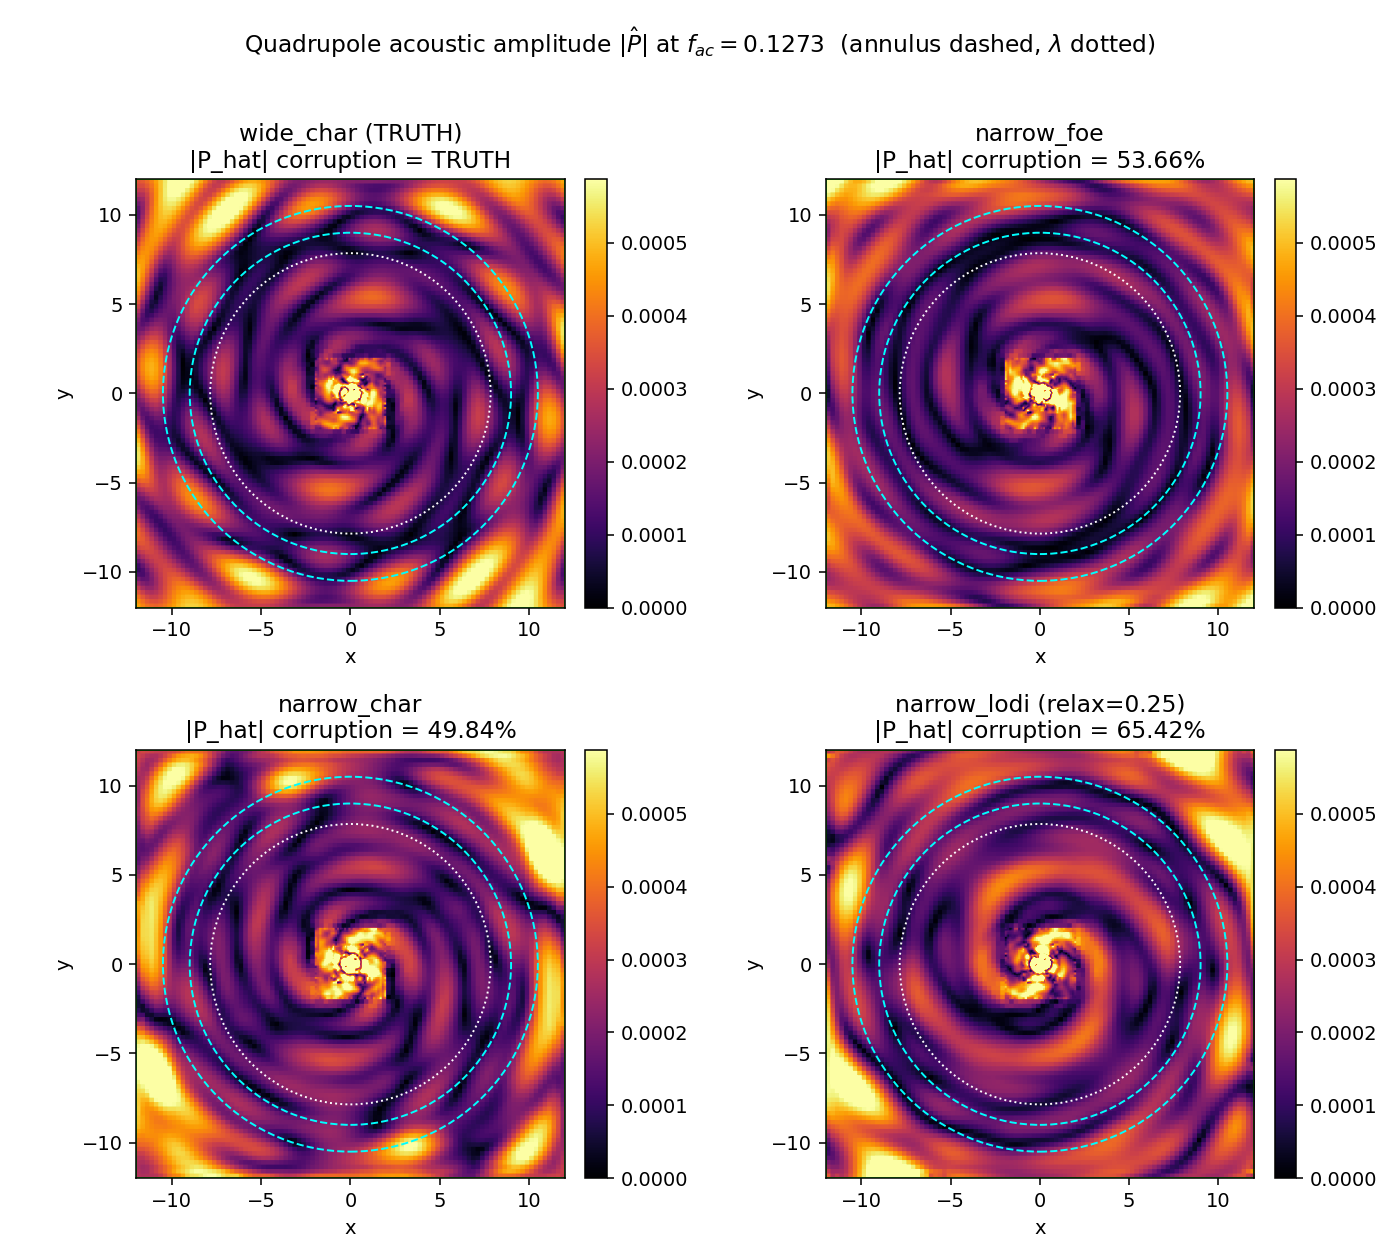
\includegraphics[width=0.86\textwidth]{figures/cvp_pHat_quadrupole.png}
\caption{Quadrupole acoustic amplitude $|\hat P|$ at $f_{\text{ac}}=0.1273$ for
the four runs (annulus dashed, $\lambda$ dotted). The truth and the three
truncated-domain BCs are visually near-identical spirals; the quoted percentages
are the annulus-$L^2$ amplitude corruptions, all near the $64\%$ noise floor.}
\label{fig:cvpphat}
\end{figure}

\begin{figure}[h]\centering
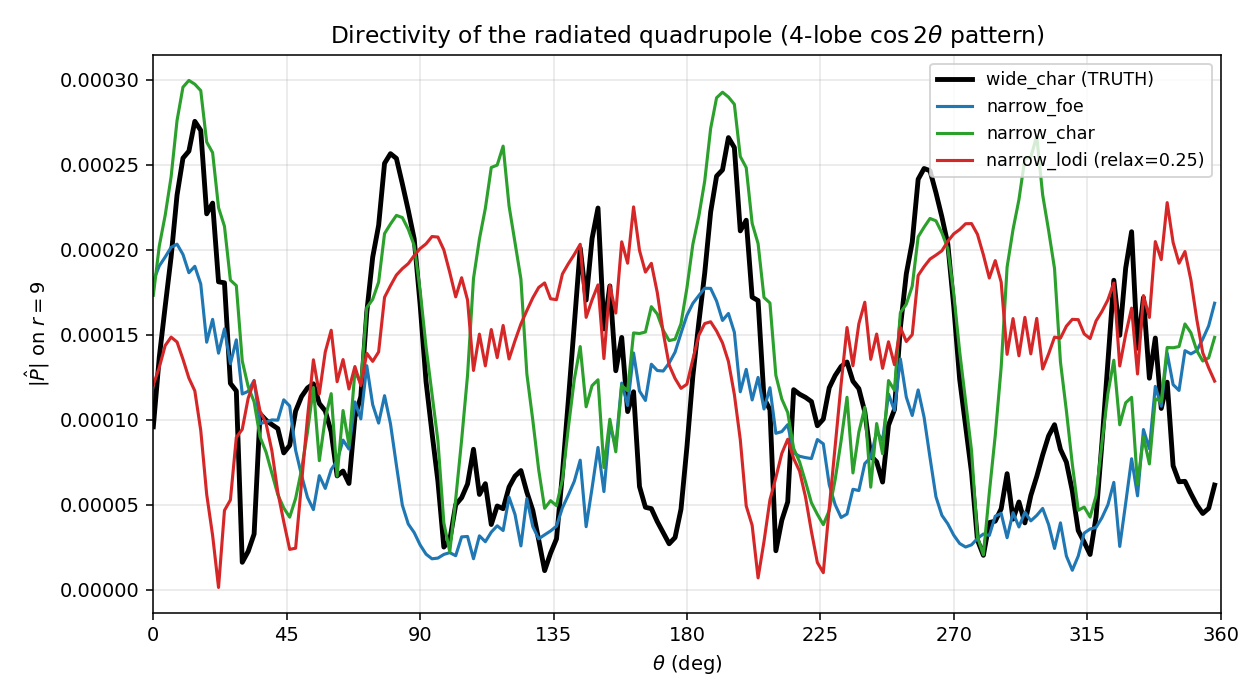
\includegraphics[width=0.74\textwidth]{figures/cvp_directivity.png}
\caption{Directivity $|\hat P|(\theta)$ on $r=9$. The trace is dominated by
spiral-arm crossings and residual near field, not a clean $\cos2\theta$
quadrupole lobe pattern, and the four BCs trace curves of the same magnitude ---
visual confirmation that the wave does not discriminate them.}
\label{fig:cvpdir}
\end{figure}

\paragraph{The one clean discriminator is mean anchoring.} The only field-level
difference that exceeds its noise is the DC mode --- the far-field mean pressure,
a weak ($<1\%$ of $p_0$) effect. Over the window the annulus-mean drift is
$-8\times10^{-5}$ (foextrap) $\approx +1.4\times10^{-4}$ (char)
$\ll +7.2\times10^{-3}$ (LODI), and the absolute far-field mean offset is
smallest for char ($\approx$ wide), then foextrap, then LODI. This both
reproduces the 1-D reflection/anchoring trade-off and \emph{settles the
fair-LODI question}: a finite relaxation $\sigma_p=0.25$ does \emph{not} win on
the wave (it is the noisiest) and \emph{under-anchors} the mean (largest residual
drift). Its advertised ``low reflection $+$ anchoring'' is not realised here,
because at near-normal incidence the simplest \texttt{foextrap} is already
non-reflecting and the corrected characteristic anchors the mean as well without
a relaxation term.

\paragraph{Conclusion of the 2-D test.} The co-rotating vortex pair is a clean
\emph{negative control}. With a rigorous, drift-free, phase-aware,
floor-calibrated metric it confirms that there is \emph{no} dramatic
non-reflecting-BC advantage for free acoustic radiation: \texttt{foextrap}
radiates the quadrupole spiral as cleanly as the characteristic and LODI
closures, and every BC difference on the wave lies below the measurement floor.
The genuine, \emph{dramatic} advantage of the characteristic far-field is
elsewhere --- mean-state anchoring and, above all, the crossing of an oblique
strong shock through the boundary, where the corrected code 7 enables a
$\sim2.5\times$ lateral-domain reduction that \texttt{foextrap} cannot survive
(companion cylinder side-domain study).

\section{Recommendation for the validation cases}
\begin{table}[h]\centering\small
\begin{tabular}{@{}lll@{}}
\toprule
Boundary & Local $M_n$ & Best choice \\
\midrule
streamwise inflow (all cases) & $\le-1$ supersonic & any (all identical, exact) \\
streamwise outflow (all cases) & $\ge+1$ supersonic & any (all identical, exact) \\
lateral far-field (all cases) & $\approx 0$ & \textbf{foextrap (2)} \\
\bottomrule
\end{tabular}
\caption{Recommended far-field BC per boundary.}
\end{table}

\noindent
\textbf{Practical conclusions.}
\begin{enumerate}
\item On every \emph{streamwise} boundary the flow is supersonic, so
\texttt{foextrap}, Dirichlet and algebraic NSCBC reduce to the identical
exact closure (full extrapolation at outflow, full prescription at inflow).
Mean loads ($C_d$, $C_p$) are therefore BC-independent, consistent with the
measured cylinder $\langle C_d\rangle$ agreeing to $<0.2\%$ across BCs.
\item On the \emph{lateral} far-field ($M_n\!\approx\!0$) the algebraic
``NSCBC'' reflects $\sim\!78\%$ of a normally incident acoustic wave;
\texttt{foextrap} does not, passes post-shock states (hard Dirichlet would force
freestream onto the post-shock gas where the bow shock crosses the boundary),
and lets entropy/vorticity leave. \texttt{foextrap} (code \texttt{2}) is the best
available lateral choice. Its only weakness --- it does not anchor the mean
pressure --- is harmless here because the \emph{supersonic inflow} pins the
global state; in a closed or subsonic problem one would instead need the
anchoring of a relaxed NSCBC. The sphere cases already use \texttt{foextrap} on
the lateral faces; the cylinder uses NSCBC (code \texttt{7}) there and is the one
case whose schlieren shows lateral acoustic artefacts.
\item The algebraic ``NSCBC'' is \emph{not buggy} --- it is a correct
steady-state far-field that is reflective for unsteady waves because it omits
the relaxation term. For unsteady/aeroacoustic work a proper
characteristic-flux NSCBC would have to be added.
\end{enumerate}

\end{document}
